% -*- coding: utf-8 -*-
% !TEX program = xelatex


\chapter{图片的使用}


\section{简单图片}

\begin{figure}[!htbp]
    \centering
    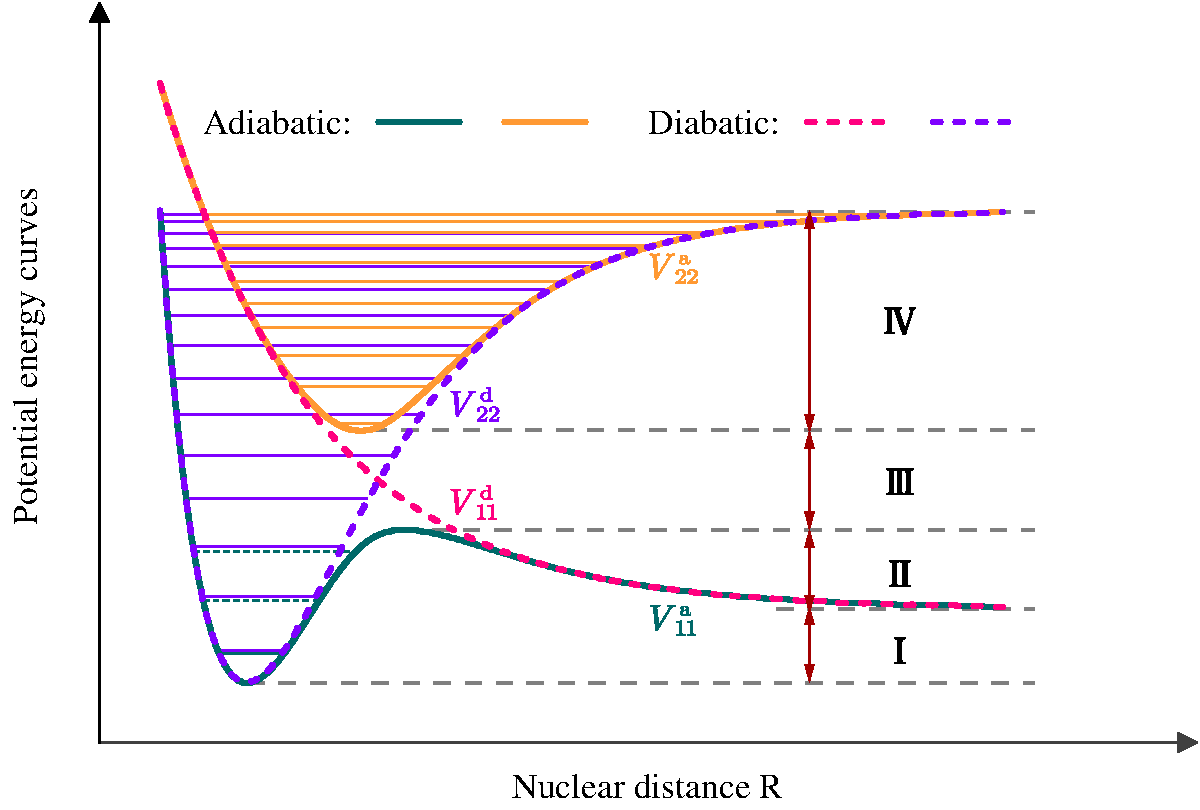
\includegraphics[width=0.5\linewidth]{pic/njpFigure1.pdf}
    \bicaption{绝热和非绝热表示中的典型势能曲线}{Typical potential energy curves in the adiabatic and diabatic representations}
    \label{fig:example}
\end{figure}


\section{进阶拼图}


\begin{figure}[!htbp]
    \centering
    \subfloat[势形共振]{\label{fig:shape}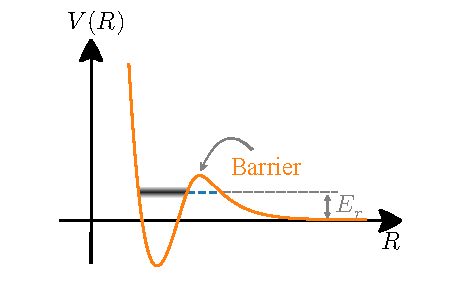
\includegraphics[width=.45\textwidth]{pic/Intro-pic_shape1.pdf}} \qquad
    \subfloat[Feshbach共振]{\label{fig:feshbach}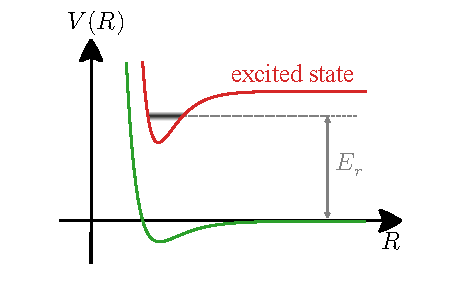
\includegraphics[width=.45\textwidth]{pic/Intro-pic_feshbach1.pdf}}
    \bicaption[势形共振和Feshbach共振示意图]{势形共振和Feshbach共振示意图}{Schematic for shape and Feshbach resonance}
    \label{fig:shapeandfeshbach}
\end{figure}